% Preamble
% ---
\documentclass[a4paper]{article}

% Packages
% ---
\usepackage{amsmath} % Advanced math typesetting
\usepackage[utf8]{inputenc} % Unicode support (Umlauts etc.)
\usepackage[ngerman]{babel} % Change hyphenation rules

\usepackage{amssymb}
\usepackage{hyperref} % Add a link to your document
\usepackage{graphicx} % Add pictures to your document
\usepackage{tabularx}
\newcolumntype{C}[1]{>{\centering\arraybackslash}p{#1}}
\usepackage{listings} % Source code formatting and highlighting
\usepackage[inline]{enumitem}
\usepackage{fullpage} %weiniger abstand zu den seiten
%Code
\usepackage{color}
\usepackage{colortbl}
\usepackage{textcomp}
\definecolor{listinggray}{gray}{0.9}
\definecolor{lbcolor}{rgb}{0.9,0.9,0.9}
\lstset{
	backgroundcolor=\color{lbcolor},
	tabsize=4,
	rulecolor=,
	basicstyle=\scriptsize,
	upquote=true,
	aboveskip={1.5\baselineskip},
	columns=fixed,
	showstringspaces=false,
	extendedchars=true,
	breaklines=true,
	prebreak = \raisebox{0ex}[0ex][0ex]{\ensuremath{\hookleftarrow}},
	frame=single,
	showtabs=false,
	showspaces=false,
	showstringspaces=false,
	identifierstyle=\ttfamily,
	keywordstyle=\color[rgb]{0,0,1},
	commentstyle=\color[rgb]{0.133,0.545,0.133},
	stringstyle=\color[rgb]{0.627,0.126,0.941},
}

\begin{document}

\author{Anleitung und Sicherheitsinformationen} % The authors name
\title{SIGMA R19 \\ Independent Dual Extruder}
\date{\today{}} % Sets date you can remove \today{} and type a date manually
\maketitle{} % Generates title
\section{Nutzungsberechtigung}
Dieses Gerät darf nur mit einer gültigen \textbf{Geräteeinweisung und Sicherheitsbelehrung} genutzt werden. Bei Fragen oder Problemen wendet euch an einen Betreuer.
\section{Gefahrenhinweise}
\begin{center}
	\begin{tabular}{C{5cm}C{5cm}C{5cm}}
		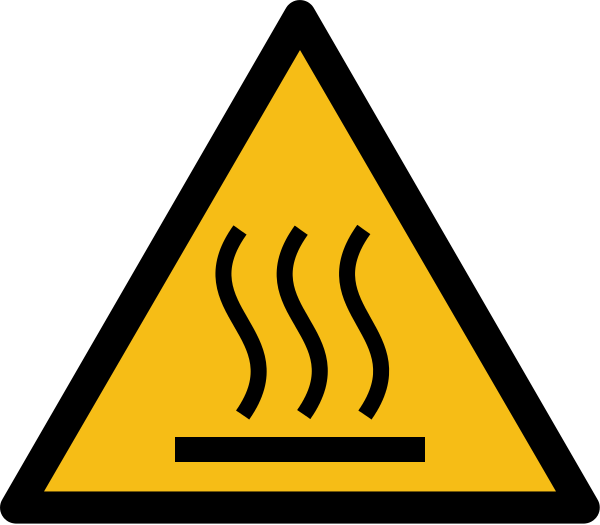
\includegraphics[width=2.5cm]{hot-surface.png} & 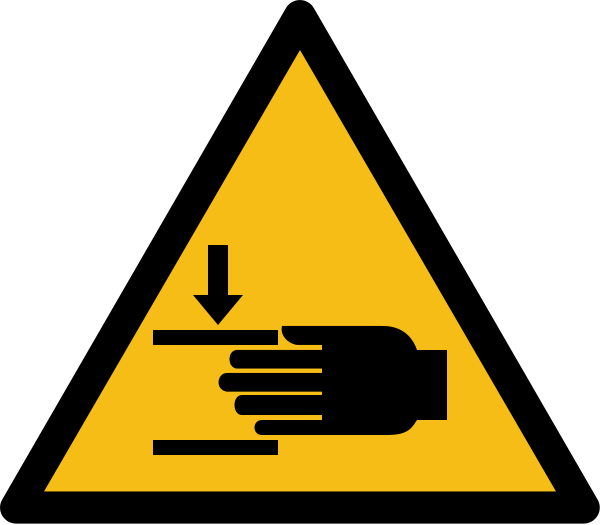
\includegraphics[width=2.5cm]{hand-injury.png} & 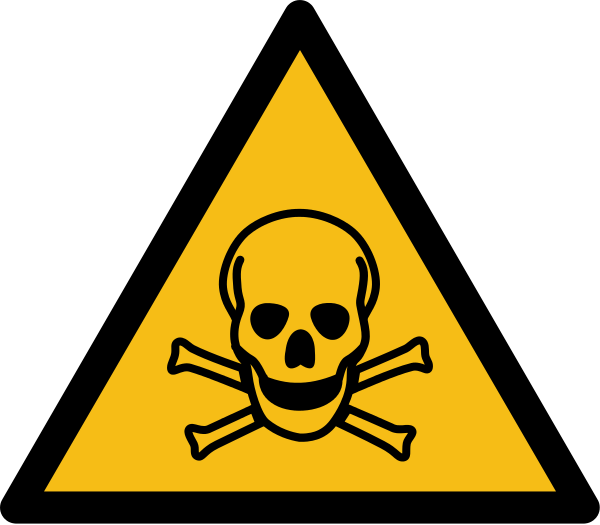
\includegraphics[width=2.5cm]{toxic.png}\\
		\textbf{Achtung heiße Oberfläche!} & \textbf{Achtung Quetschgefahr!} & \textbf{Achtung Giftig!}
	\end{tabular}
\end{center}

		
 Sowohl die Druckplatte als auch die Druckspitzen werden mit 100-290°C sehr heiß!
 Lasse also erst alles Abkühlen bevor du die Druckplatte oder Spitzen reinigen willst.
 I.d.R dauert dies unter 7 Minuten.\\\\
Im 3D-Drucker sind viele bewegliche Teile! Während des Druckvorgangs haben Hände, Haare, Schals o.ä nichts im Drucker zu suchen.\\\\
Die Druckmaterialien sind nicht unschädlich und geben teilweise giftige Dämpfe ab. Lüfte den Raum regelmäßig, insbesondere während langer Druckaufträgen. Atme beim Drucken nicht näher als 25 cm vom Werkzeugkopf entfernt.\\\\
Im Falle eines Notfalls, ist es sollte die Stromversorgung des Geräts zu unterbrochen werden. Ziehe hierfür den Stecker auf Fensterseite des Raumes. 
\section{Technische Daten}
 \begin{tabular}{|l|l|}
 	\hline
 	Hersteller & BCN3D\\
 	\hline
 	Leistung & 240W \\
 	\hline
 	Anzahl Köpfe & 2 \\
 	\hline
	Druckvolumen &  210 x 297 x 210mm\\
	\hline
	Layerdicke & 0.05 - 0.5mm\\
	\hline
	Filament Durchmesser & 2.85 ± 0.05 mm\\
	\hline
	Filament Material & PLA / ABS / Nylon / PET-G / TPU / PVA\\
	\hline
	Lautstärke & 50 dBA\\
	\hline
	Kompatible Dateien & gcode \\
	\hline
\end{tabular}
\newpage
\section{Bedienung}
\subsection{Allgemeines}
Falls es kälter als 15 oder wärmer als 35 °C ist, direkte \textbf{Sonneneinstrahlung} auf den Drucker nicht vermeidbar ist oder sehr \textbf{staubige Arbeiten} im Raum durchgeführt werden, darf nicht gedruckt werden.\\
Der 3D-Drucker und sein Tisch dürfen in keinem Fall bewegt werden, da sonst eine vollständige Kalibrierung von Nöten ist.\\
Die offizielle Anleitung (Englisch) findest du im Hängeregister "`3D-Drucker"' im Rollcontainer.
\subsection{Druckvorbereitung}
\begin{itemize}
	\item Die 3D-Modelle müssen im '.stl'- oder '.obj'-Format vorliegen.
	\item Das ‘Slicen’, also dem Erstellen der für 3D-Drucker lesbaren '.gcode',  geschieht mit der Software 'BCN3D Cura' und dem Custom-Profil 'fast with brim' oder 'standart with brim'. Die Profile sind auf dem Werkstatt-Github Repo\footnote{\url{https://github.com/fsi-tue/Werkstatt}} zu finden.
	Je nach 3D-Modell empfiehlt sich eine andere Voreinstellung zu nutzen. Spreche dies mit einem Betreuer oder einer anderen erfahrenen Person ab.\\
	Gegebenenfalls müssen Einstellungen wie Unterstützungsstrukturen und Wandstärke verändert werden.
	\item Klicke nun auf "`Prepare"' unten rechts. Nun sollte angezeigt werden wie lange der Druckauftrag voraussichtlich dauert. Rechne $\approx 15\%$ mehr ein.
	\item Bei längeren Druckaufträgen \textbf{($\geq$30 min)} sollte die .gcode Datei auf einer SD-Karte gespeichert werden. Diese findest du auf der Vorderseite des Druckers. Der Dateiname sollte mit deinem Namen beginnen. Bsp.:Julia\_Musterfrau\_Adapter.gcode\\
	\textbf{Während des Drucken über USB darf weder die Verbindung unterbrochen, noch ein weiteres BCN3D Cura Fenster geöffnet werden}
\end{itemize}
\subsection{Drucken}
\begin{itemize}
	\item Schalte den 3D-Drucker an. (Schalter befindet sich auf der linken Seite)
	\item Klebe auf die Glasplatte eine Schicht 'Yellow-Tape'. Diese Bahnen sollten überlappungsfrei sein.
	\item Heize den genutzten Druckerkopf und die Platte vor.
	\item Führe eine Y-Achsenkalibrierung durch. "`Utilities  $\rightarrow$ Calibration $\rightarrow $Printing Surface Calibration"'
	\item SD-Karte einführen und Druckauftrag im Menu "`Print"' auswählen oder am PC starten.
	\item Warten und Beobachten. Sollten in den kritischen ersten 10 Minuten (bzw. ersten paar Layer )etwas schiefgehen musst du den Auftrag abbrechen bzw. pausieren. Es ist möglich dein Druck zu retten, spreche ggf. mit einem Betreuer.
\end{itemize}
\subsection{Nach dem Druck}
\begin{itemize}
	\item Warte mit die Druckplatte sich abgekühlt hat. Dies sollte nach 1 Minuten soweit sein.
	\item Entferne dein Werk vorsichtig. Sollte es sich nicht einfach von der Platte lösen, kannst du ein Spachtel nutzen. Achte darauf das 'Yellow-Tape' nicht zu verkratzen.
	\item Falls das Tape doch beschädigt ist, entferne alles.
	\item Nun kannst du den Drucker ausschalten. (Schalter auf der linken Seite)
\end{itemize}
\end{document}
